\documentclass{article}
\usepackage{graphicx} % Required for inserting images
\usepackage{amsmath}
\usepackage[a4paper, total={6in, 8in}]{geometry}
\usepackage[font=small,labelfont=bf]{caption}
\title{PHYS414 - Final Project}
\author{
    Cem Cengiz Yazıcı \\
    Department of Physics, Koç University \\
    0076272 \\
    Rumelifeneri Yolu, 34450 Sariyer, Istanbul, Turkey
}
\date{(Dated: January 10, 2025)}


\begin{document}

\maketitle

\begin{center}
    \section*{I. Newtonian Solution of a Star}
\end{center}

\subsection*{A. Lane-Emden Equation}
If we start with hydrostatic equilibrium of stars in Newtonian gravity, we can obtain following ODEs:
\begin{equation}
    \frac{m(r)}{dr} = 4\pi r^2\rho(r) 
\end{equation}
\begin{equation}
    \frac{dp(r)}{dr} = \frac{-Gm(r)\rho (r)}{r^2}
\end{equation}
$p(r)$ and $m(r)$ notates the mass of star within the radius r and the density respectively. Using (2), we can solve for m(r) and take its derivative respect to r:
\begin{equation}
    -\frac{dm(r)}{dr} = \frac{d}{dr}(\frac{r^2}{G\rho(r)}\frac{dp(r)}{dr}) 
\end{equation}

We can use the equation for $\displaystyle\frac{dm(r)}{dr}$ in (1) and get:

\begin{equation}
    \frac{1}{4\pi r^2}\frac{d}{dr}(\frac{r^2}{G\rho(r)}\frac{dp(r)}{dr}) = -\rho(r)
\end{equation}

Assuming polytropic equation of state, we can $P$ and $\rho$ by the relation:
\begin{equation}
    p = K\rho ^\gamma = K\rho ^{1+\frac{1}{n}}
\end{equation}
where in is defined as polytropic index. If we take the r derivative of $p(r)$:
\begin{equation}
    \frac{dp(r)}{dr} = \frac{(n+1)}{n}K\rho^{\frac{1}{n}}\frac{d\rho(r)}{dr}
\end{equation}
We can see that it is helpful to define a parameter $p = p_c\theta^n$ for simplicity. Now, plugging the expression for $p(r)$ into (6) into (4), we get:
\begin{equation}
    (\frac{K}{G})(n+1)(p_c^{\frac{1-n}{n}})(\frac{1}{4\pi r^2})\frac{d}{dr}(r^2\frac{d\theta(r)}{dr}) = -\theta^n(r)
\end{equation}
Now, lets define a constant $A$ and scaled radius $\xi$:

\begin{equation}
    A^2 = \frac{(n+1)K\rho_c^{\frac{1}{n} -1}}{4 \pi G}
\end{equation}

\begin{equation}
    \xi = r/A
\end{equation}
So that hydro-static EOS can be neatly written in the desired form:
\begin{equation}
    \frac{1}{\xi^2}\frac{d}{d\xi^2}(\xi^2\frac{d\theta(\xi)}{d\xi}) + \theta^n = 0
\end{equation}

If we employ Mathematica for exact solution, we get:
\begin{equation}
    \theta(\xi) = -\frac{i e^{-i \xi} \left(-1+e^{2 i \xi}\right)}{2 \xi}
\end{equation}
which has regular solutions at the center:
\begin{equation}
    \theta(\xi) = 1 - \frac{1}{6}\xi^2 + \frac{1}{120}\xi^4 + O(\xi^6) + ... ,
\end{equation}

Furthermore, we can obtain the total mass by integrating (1) but now with scaled parameters:
\begin{equation}
    M_{total} = 4\pi A^3p_c\int_{0}^{R_{max}/A}\theta^n(\xi)\xi^2d\xi
\end{equation}
Using (10), We can replace $\theta^n(\xi) \xi^2$ with $\frac{d\theta(r)}{d\xi}\xi^2$ and get:

\begin{equation}
    M_{total} = -4\pi A^3p_c\frac{1}{\xi}\frac{d\theta(\xi)}{d\xi}
\end{equation}

Using the definition of $A$, we can substitute the expression for $p_c$ and obtain a relation of M and R.
\begin{equation}
    -4\pi R^3(\frac{4\pi G A^2}{K(n+1)})^{n/(1-n)}\frac{d\theta(\xi)}{d\xi}
\end{equation}
Employing the definition $R = A\xi_n$:
\begin{equation}
    M_{total} = -R^{\frac{3-n}{1-n}} (-4\pi)(\frac{4\pi G}{K(n+1)})^{n/(1-n)}\frac{d\theta(\xi_n)}{d\xi_n}\xi_n^{\frac{n+1}{n-1}}
\end{equation}
Where $M_{total}$ can we written as a product of a constant $\beta$ and $R^{\frac{3-n}{1-n}}$:
\begin{equation}
    M_{total} = \beta R^{\frac{3-n}{1-n}}
\end{equation}
thus, we end up with an relation for group of stars that share same polytropic EOS:
\begin{equation}
    M_{total} \propto R^{\frac{3-n}{1-n}}
\end{equation}

\newpage
\subsection*{B. White Dwarf Data Visualisation}
Using the white dwarf data and plot M (in solar mass unit) and R (in earth radius units), we get:
\begin{center}
    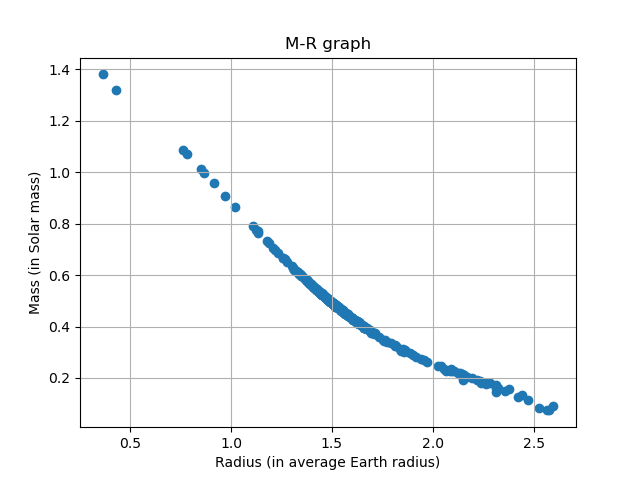
\includegraphics[scale=0.65]{images_newton/1_M_vs_R_fitered.png}
    \captionof{figure}{White Dwarf Data Visualization}
\end{center}

\subsection*{C. Low-Mass White Dwarves}
For a white dwarf, we can express the EOS which is dominated by the electron degeneracy:
\begin{equation}
    P = C[x(2x^2-3)(x^2+1)^{1/2}+3sinh^{-1}x],
\end{equation}
\begin{equation}
    X = (\frac{\rho}{D})^{\frac{1}{q}}
\end{equation}
Using mathematica, we can analytically calculate the taylor series of equation (20) for $|x|<<0$:
\begin{equation}
    \frac{8 C x^5}{5}-\frac{4 C x^7}{7}+\frac{C x^9}{3}-\frac{5 C x^{11}}{22}+O\left(x^{12}\right)
\end{equation}
Omitting higher order terms, we get $P = \frac{8 C x^5}{5}$. We can identify $n_*$ term in \begin{equation}
    P=K_*\rho^{1+\frac{1}{n_*}}
\end{equation}
as
\begin{equation}
    n_* = q/(5-q).
\end{equation}
We can obtain a linear relation between $ln(M)$ and $ln(B)$ and apply a linear fit to calculate the slope for filtered data ($ln(M) > 0.25$):
\begin{center}
    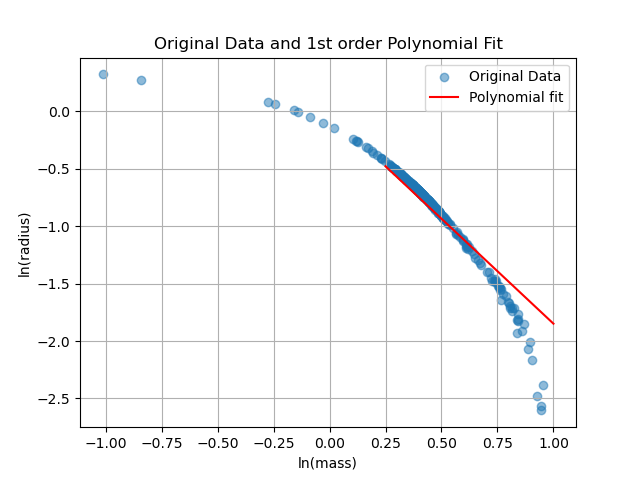
\includegraphics[scale=0.65]{images_newton/2_Polyfit.png}
    \captionof{figure}{1st order polynomial fit applied to the R and M ( $ln(M) > 0.25$).}
\end{center}
From the fit, we can calculate the slope and use the relation for $n_*$ as follows:
\begin{equation}
    slope = \frac{3-n_*}{1-n_*} = -3.3387
\end{equation}
From theory, we assume $q$ is an integer and find that smallest positive integer satisfying (23) is $q=3$, which gives $n=1.5$. Now, we can calculate the Lane-Emden equation and obtain unknown parameters:
\begin{align}
    &\xi  = 3.6578223569228965 \\
    &\theta	=	1.0176017680895436e^{-16} \\
    &\theta '(\xi)	=	-0.202860682607365 \\
\end{align}
We can now calculate $K_*$ since we already have an explicit formula (eq. (16)) for $K_*$ in terms of $\xi$ and $\theta ' (\xi)$.
\begin{align}
    &K_* = 0.030964561408303514
\end{align}
Moreover, we can calculate $p_c$ since we know $\xi$ and $\theta'(\xi)$. Using equation (14) results:
\begin{equation}
    \rho_c = -\frac{M\xi}{4\pi R^3(\theta '(\xi))}
\end{equation}
\newpage
Using (30), we can plot $\rho_c$ vs. $M$ graph:
\begin{center}
    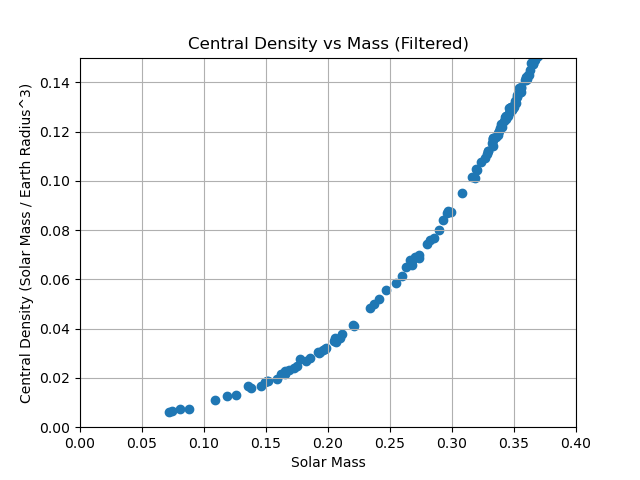
\includegraphics[scale=0.65]{images_newton/3_rhoc_vs_M.png}
    \captionof{figure}{Low-Mass White Dwarf: Central Density ($\rho_c$) vs Mass in logarithmic base.}
\end{center}
\begin{center}
  \section*{II. Einstein}  
\end{center}

\subsection*{A. Mass vs. Radius}

\begin{center}
    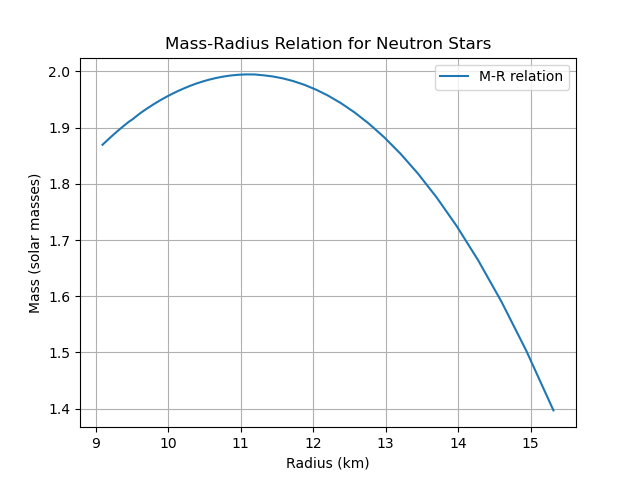
\includegraphics[scale=0.65]{images_einstein/e1_mass_vs_radius.png}
    \captionof{figure}{Mass vs. Radius with differing $\rho_c$}
\end{center}
50 $\rho_c$ values are sampled between $10^{-3}$ and $9 \times10^{-3}$. Resulting Relation can be seen in Figure 4.

\subsection*{B. Fractional Binding Energy}
We have the following relation for baryonic mass:
\begin{equation}
    m'_P = 4\pi \left(1 - \frac{2m}{r}\right)^{-\frac{1}{2}} \, r^2 \rho
\end{equation}
where we can define fractional binding energy ($\Delta$) as:
\begin{equation}
    \Delta \equiv \frac{M_P - M}{M}.
\end{equation}
and obtain the relation in Figure 5.
\begin{center}
    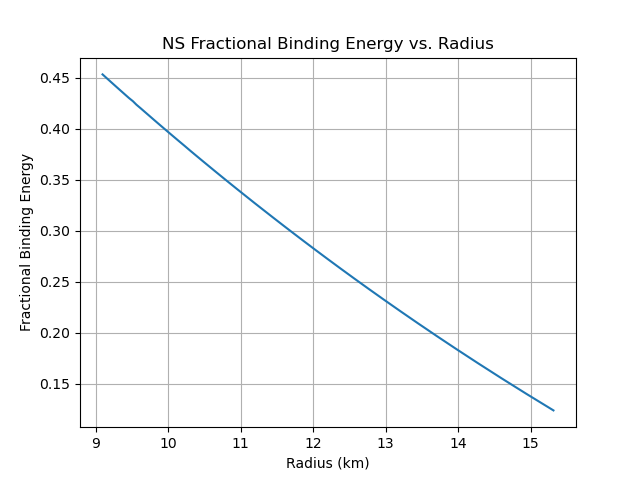
\includegraphics[scale=0.65]{images_einstein/e2_frac_binding_energy.png}
    \captionof{figure}{$\Delta$ vs radius $R$}
\end{center}
where we can observe that the relation is highly linear.
\subsection*{C. Mass vs Central Density ($\rho_c$)}
Let's begin with simple criterion for NS stability:
\begin{gather}
    \frac{dM}{d\rho_c} > 0 \quad \longrightarrow \quad \text{stable} \\
    \frac{dM}{d\rho_c} < 0 \quad \longrightarrow \quad \text{unstable}    
\end{gather}
Overall, $\frac{dM}{d\rho_c} >0$, otherwise it forms a black hole. If we visualize $M$ vs $\rho_c$:
\begin{center}
    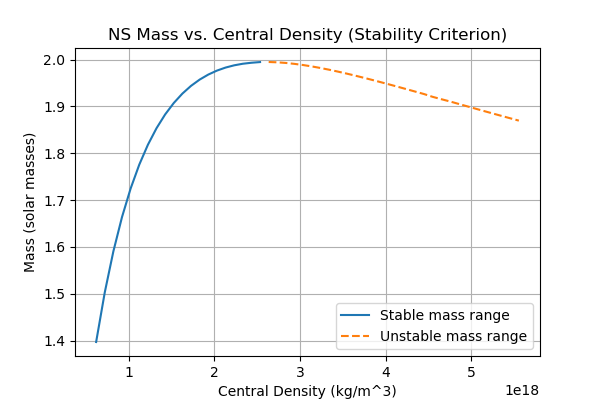
\includegraphics[scale=0.65]{images_einstein/e3_M_vs_rhoc.png}
    \captionof{figure}{Numerically calculated stable and unstable regions for a Neutron Star}
\end{center}
Moreover, we can obtain the maximum allowed mass for NS:
\begin{equation}
    M_{max} = 1.9947289179622747
\end{equation}

\subsection*{D. Maximum Allowed Mass vs Polytropic Coefficient $K$}
Since we know maximum allowed mass $M^{*}$ depends on the EOS, we can calculate $M^{*}$ using fixed polytropic index. We can iterate over $\rho_c$ values for a single $K$ value to solve the TOV. Then, we repeat process for all selected $K$ values to find maximum allowed mass.

\begin{center}
    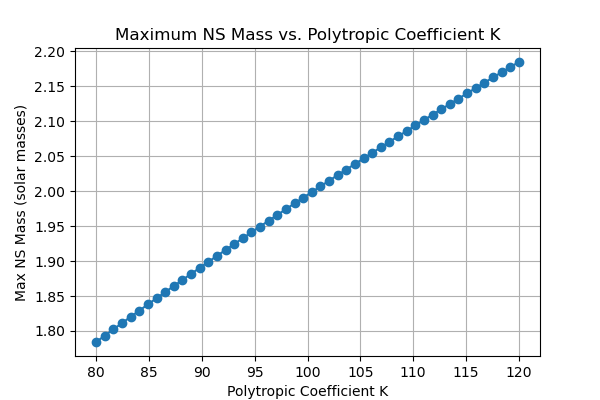
\includegraphics[scale=0.65]{images_einstein/e4_max_allowed_mass_eos.png}
    \captionof{figure}{Maximum Allowed Mass $M^{*}$ vs polytropic index $K^{*}$}
\end{center}
If we apply cubic interpolation to the data of Figure 7 and leverage root finding using the mass of biggest observed neutron star $M = 2.14$, we get the maximum allowed value of $K$:
\begin{equation}
    K = 115.0947205875922
\end{equation}

\end{document}
